\documentclass[aspectratio=169]{beamer}
\usetheme{Madrid}
\usepackage{graphicx}
\usepackage{booktabs}

\title{Branch Specialization in Attention}
\subtitle{Toy Local-vs-Induction Competition Checkpoint}
\author{Research checkpoint}
\date{May 22, 2026}

\begin{document}

\begin{frame}
  \titlepage
\end{frame}

\begin{frame}{Current Question}
  \textbf{Stronger RQ5 test:} Does heterogeneous head dimension produce a
  stable role partition under task competition?

  \vspace{0.7em}
  Desired positive result:
  \[
    \text{small heads} \rightarrow \text{local role}, \quad
    \text{large head} \rightarrow \text{global induction role}
  \]

  \vspace{0.7em}
  This clean result did not appear.
\end{frame}

\begin{frame}{Task}
  Each sequence has two scored regions.

  \vspace{0.5em}
  Local:
  \[
    [x,\mathrm{SEP},x]
  \]
  At SEP, predict the immediately previous token \(x\).

  \vspace{0.5em}
  Induction:
  \[
    [y_1,\ldots,y_{16},y_1,\ldots,y_{16}]
  \]
  At the second \(y_i\), predict \(y_{i+1}\).
\end{frame}

\begin{frame}{Experimental Arms}
  \begin{table}
    \centering
    \begin{tabular}{lll}
      \toprule
      Config & Head dimensions & Purpose \\
      \midrule
      uniform4 & [32,32,32,32] & same-head-count baseline \\
      hetero4 & [16,16,32,64] & heterogeneous intervention \\
      uniform2 & [64,64] & fewer/wider control \\
      64-first & [64,16,16,32] & position control \\
      \bottomrule
    \end{tabular}
  \end{table}

  All models use two layers, \(d_{model}=128\), five seeds, and total attention
  dimension \(128\).
\end{frame}

\begin{frame}{Both Objectives Learn}
  \begin{table}
    \centering
    \begin{tabular}{lrr}
      \toprule
      Config & Local acc. & Induction acc. \\
      \midrule
      uniform4 & 1.0000 & 0.9999 \\
      hetero4 & 1.0000 & 0.9992 \\
      uniform2 & 1.0000 & 0.9976 \\
      64-first & 0.9999 & 0.9986 \\
      \bottomrule
    \end{tabular}
  \end{table}

  The role comparison is not primarily a task-failure artifact.
\end{frame}

\begin{frame}{Role Concentration}
  \centering
  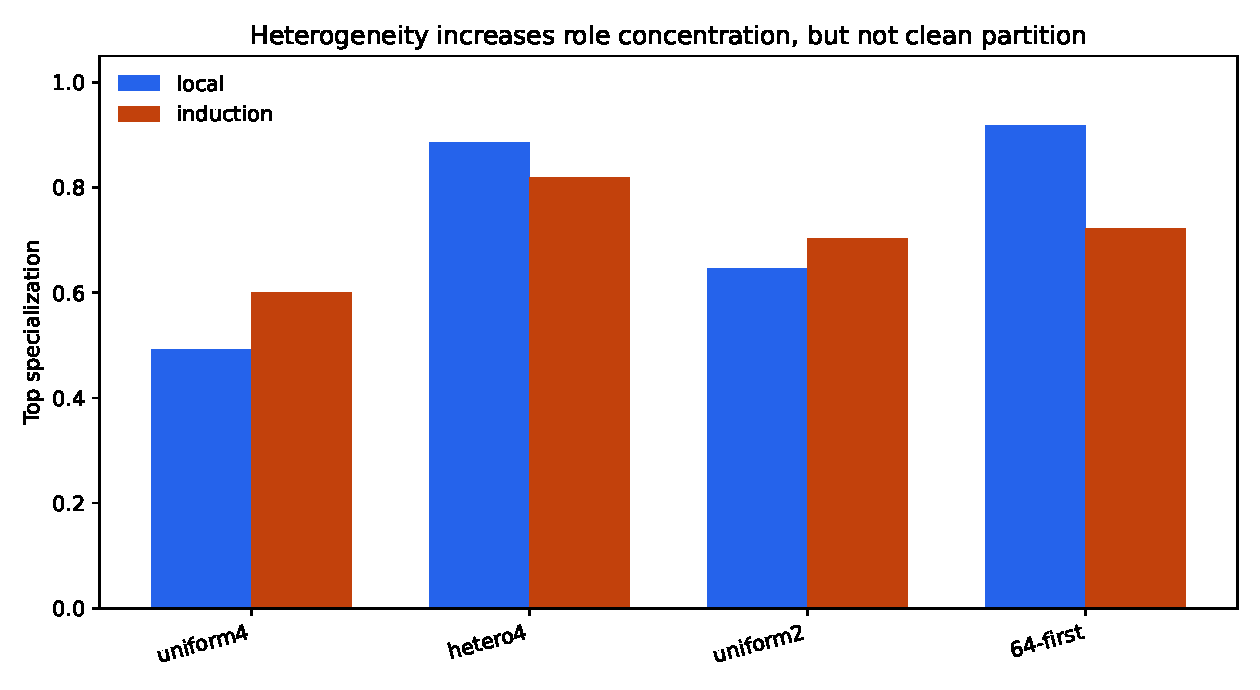
\includegraphics[width=0.88\linewidth]{figures/role_specialization.pdf}
\end{frame}

\begin{frame}{Causal Load}
  \centering
  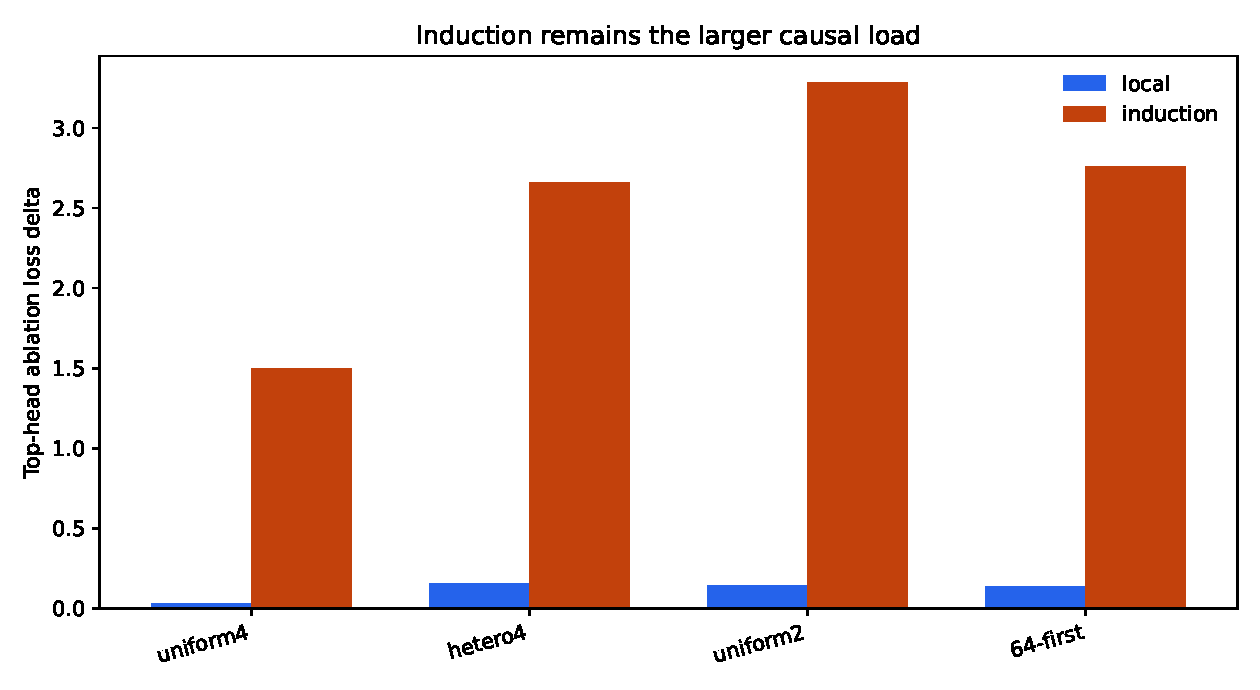
\includegraphics[width=0.88\linewidth]{figures/role_ablation_delta.pdf}
\end{frame}

\begin{frame}{Role Overlap}
  \centering
  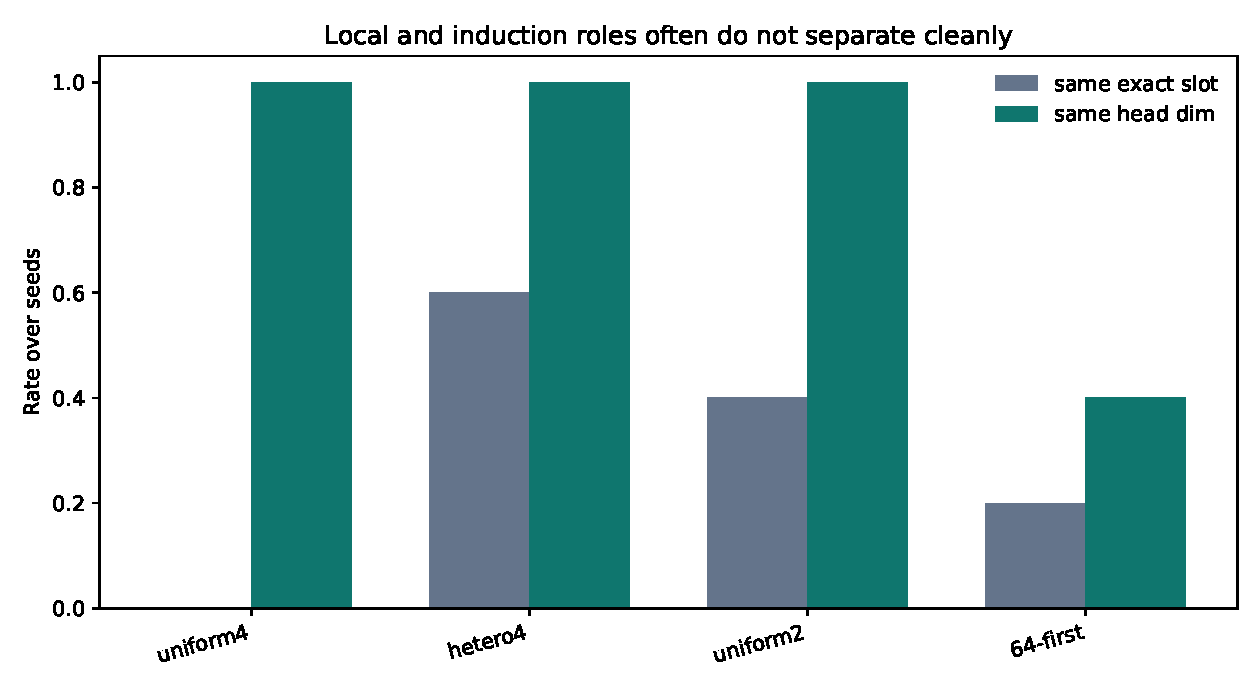
\includegraphics[width=0.88\linewidth]{figures/role_overlap.pdf}
\end{frame}

\begin{frame}{Top Dimensions}
  \centering
  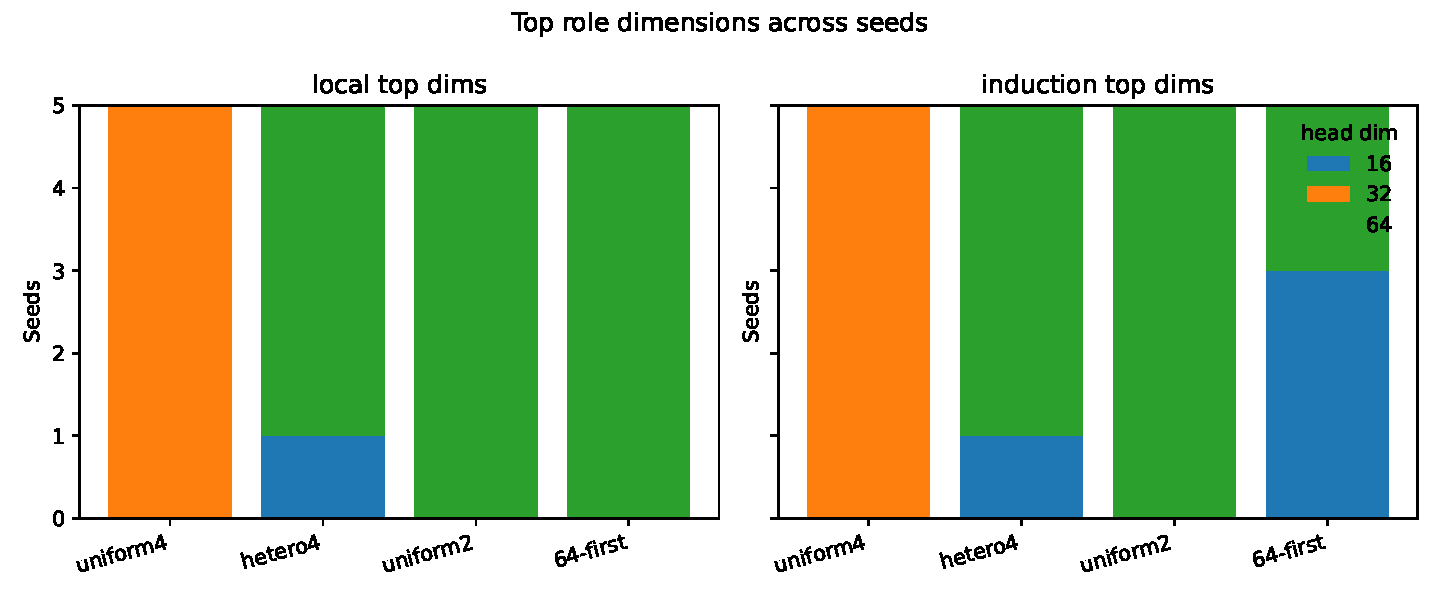
\includegraphics[width=0.88\linewidth]{figures/top_dim_counts.pdf}
\end{frame}

\begin{frame}{Layout Sensitivity}
  \centering
  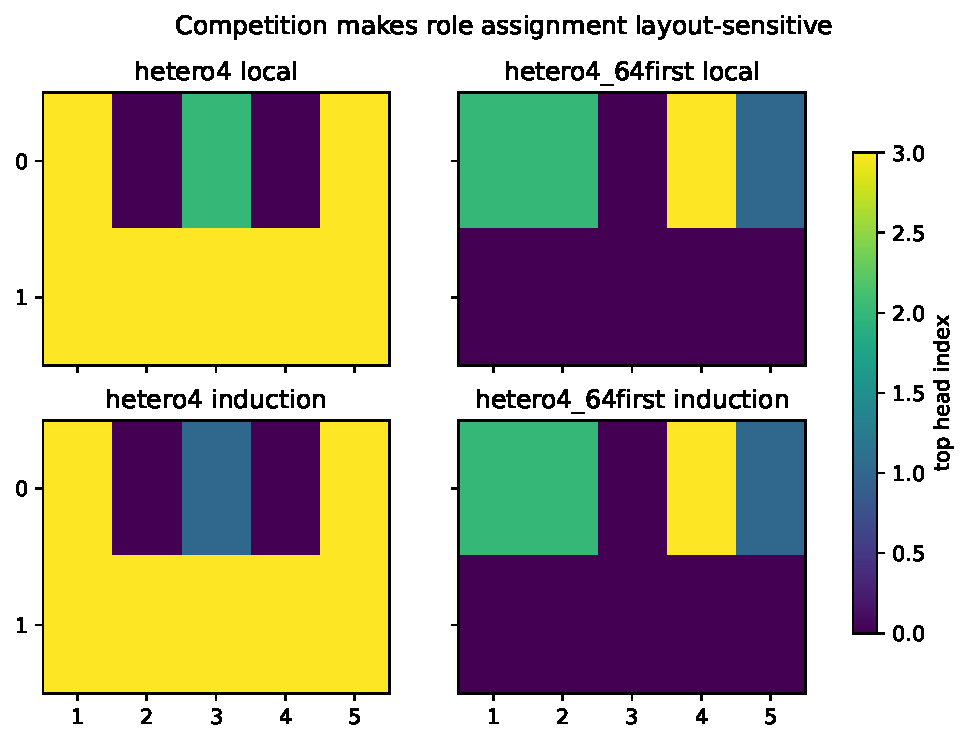
\includegraphics[width=0.88\linewidth]{figures/hetero_top_slots.pdf}
\end{frame}

\begin{frame}{Interpretation}
  Still supported:
  \begin{itemize}
    \item heterogeneous head dimensions increase causal specialization concentration;
    \item heterogeneous slots break permutation symmetry relative to uniform4.
  \end{itemize}

  \vspace{0.6em}
  Not supported yet:
  \begin{itemize}
    \item small heads reliably become local heads;
    \item the large head reliably becomes the global induction head.
  \end{itemize}
\end{frame}

\begin{frame}{Decision}
  Narrow the Stage 3 claim:

  \vspace{0.6em}
  \textbf{Heterogeneity is a permutation-symmetry-breaking stabilizer, not a
  guaranteed semantic role allocator.}

  \vspace{0.8em}
  Next:
  \begin{itemize}
    \item run more heterogeneous permutations;
    \item report structure-aware slot stability;
    \item treat layout sensitivity as a real constraint on the intervention story.
  \end{itemize}
\end{frame}

\begin{frame}{Provenance}
  \begin{itemize}
    \item Script: \texttt{scripts/toy\_competition\_head\_dim\_intervention.py}
    \item Output: \texttt{results/phase3\_toy\_competition\_head\_dim\_intervention}
    \item Report: \texttt{doc/phase3\_toy\_competition\_head\_dim\_intervention.md}
    \item Data copied into this deck folder under \texttt{data/}
  \end{itemize}
\end{frame}

\end{document}
